\documentclass[a4paper]{article}
\usepackage[utf8]{inputenc}
\usepackage{enumitem}
\usepackage{tikz, pgfplots}
\usetikzlibrary{positioning}

\title{Mathematical graphics}
\author{Me}
\date{\today}

\begin{document}
	\section{Tikz}
		\tikz \draw (0,0) -- (4,0) -- (4,2) -- (0,2) -- (0,0);
	
		\vspace{0.5in}	
	
		\begin{tikzpicture}
			\draw (0,0) circle (1);
			\draw (2,0) circle (1.5in);
			\draw (5,0) ellipse (10pt and 20pt);
			\draw (5,0) ellipse (20pt and 10pt);
		\end{tikzpicture}
		
		\vspace{1in}	
	
		
\begin{tikzpicture}
			\draw (0,0) rectangle (5,4);
			\draw (0,0) grid (5,4);	
		\end{tikzpicture}
		
		\newpage
				
		The following \LaTeX{} code creates the above graphics.		
		
		%Display code in the document.
		\begin{verbatim}
			\tikz \draw (0,0) -- (4,0) -- (4,2) -- (0,2) -- (0,0);
			\vspace{0.5in}	
			\begin{tikzpicture}
				\draw (0,0) circle (1);
				\draw (2,0) circle (1.5in);
				\draw (5,0) ellipse (10pt and 20pt);
				\draw (5,0) ellipse (20pt and 10pt);
			\end{tikzpicture}
			\vspace{1in}	
			
\begin{tikzpicture}
				\draw (0,0) rectangle (5,4);
				\draw (0,0) grid (5,4);	
			\end{tikzpicture}
		\end{verbatim}

		\newpage
		
		\subsection{Drawing a circle in \LaTeX{}.}
		
			\vspace{2.5cm}
			\begin{center}
				\begin{tikzpicture}
					\draw (0,0) circle (2.5cm);
				\end{tikzpicture}
			\end{center}
		%LaTeX code for the circle	
			\begin{verbatim}
				\begin{center}
					\begin{tikzpicture}
						\draw (0,0) circle (5cm);
					\end{tikzpicture}
				\end{center}
			\end{verbatim}
			\newpage
		
		\subsection{Drawing a sphere with coloured lines and\\shading}
		
			\vspace{5cm}		
		
			\begin{center}
		
				
\begin{tikzpicture}[transform canvas={scale=4.0}]
					\draw[dashed] (0,0) -- (1,0);
					\draw (0,0) circle (1cm);
					\draw[blue] (0,-1) arc (-90:90:0.5cm and 1cm);
					\draw[dashed,red] (0,1) arc (90:270 : 0.5cm and 1cm);
					\filldraw[red] (0,1) circle (0.05cm);
					\filldraw[red] (0,-1) circle (0.05cm);
					\shade[ball color=blue!10!white,opacity=0.18] (0,0) circle (1cm);
				\end{tikzpicture}

			\end{center}
		
			\vspace{4.5cm}
					
			%LaTeX code for the sphere.
			\begin{verbatim}
				\begin{center}
					
\begin{tikzpicture}[transform canvas={scale=4.0}]
						\draw[dashed] (0,0) -- (1,0);
						\draw (0,0) circle (1cm);
						\draw[blue] (0,-1) arc (-90:90:0.5cm and 1cm);
						\draw[dashed,red] (0,1) arc (90:270 : 0.5cm and 1cm);
						\filldraw[red] (0,1) circle (0.05cm);
						\filldraw[red] (0,-1) circle (0.05cm);
						\shade[ball color=blue!10!white,opacity=0.18] (0,0) circle (1cm);
					\end{tikzpicture}
				\end{center}
			\end{verbatim}
		
		\newpage
		\subsection{Line thicknesses}
			\vspace{2cm}
			\begin{center}
			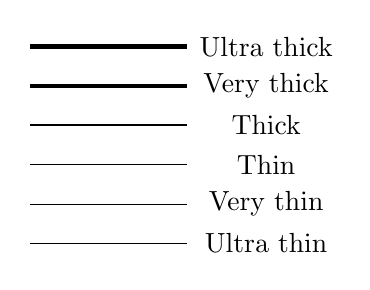
\begin{tikzpicture}
				\draw[ultra thick] (0,3) -- (2,3);
				\draw node at (3,3){Ultra thick};
				
				\draw[very thick] (0,2.5) -- (2,2.5);
				\draw node at (3,2.5){Very thick};
				
				\draw[thick] (0,2) -- (2,2);
				\draw node at (3,2){Thick};
				
				\draw[thin] (0,1.5) -- (2,1.5);
				\draw node at (3,1.5){Thin};
				
				\draw[very thin] (0,1) -- (2,1);
				\draw node at (3,1){Very thin};
				
				\draw[ultra thin] (0,0.5) -- (2,0.5);
				\draw node at (3,0.5){Ultra thin};
			\end{tikzpicture}		
			
			\end{center}

			\vspace{2cm}
			
				\LaTeX{} code for the above Tikz picture.									
			\begin{verbatim}
				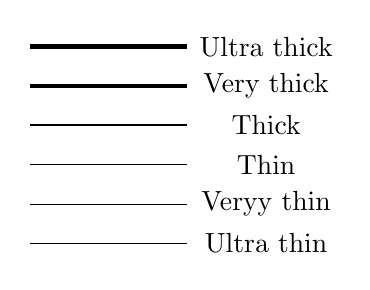
\begin{tikzpicture}
					\draw[ultra thick] (0,3) -- (2,3);
					\draw node at (3,3){Ultra thick};
				
					\draw[very thick] (0,2.5) -- (2,2.5);
					\draw node at (3,2.5){Very thick};
				
					\draw[thick] (0,2) -- (2,2);
					\draw node at (3,2){Thick};
				
					\draw[thin] (0,1.5) -- (2,1.5);
					\draw node at (3,1.5){Thin};
				
					\draw[very thin] (0,1) -- (2,1);
					\draw node at (3,1){Veryy thin};
					
					\draw[ultra thin] (0,0.5) -- (2,0.5);
					\draw node at (3,0.5){Ultra thin};
				\end{tikzpicture}		
			\end{verbatim}
		
		\newpage
		\subsection{Charts}
		
\begin{tikzpicture}[box/.style={
			rectangle,
			very thick,
			draw=black,
			font=\itshape		
		}]
		\node (label) [box] (1,-1) {Standard box};
		\end{tikzpicture}
			
				
			
		
\end{document}